\section{Traceability mega-models}\label{sec:TraceabilityMegamodels}
So far we discussed traceability and mega-modeling separate from one another in a rather abstract manner. From here upon out we will combine both by studying several real-life approaches. However, the set-theoretic notion of the MDE-Mega-Model in §\ref{subsec:TheMDEMegaModel} might have already revealed the connection between both topics. 

\subsection{MDE traceability}
MDE needs formalization in order to handle traceability properly. But the definition of traces alone does not work well with automation. Therefor the concept of \textit{traceability links} was introduced. Aizenbud-Reshef et al. define such links as \textit{''[...] any relationship that exists between artifacts involved in the software-engineering life cycle. [...]''} \cite{ModelTraceability}. Regarding models we have seen those relations in action:
\begin{center}
$a R b$
or
$(a,b) \in R$
\end{center}
This is the formalization utilized by the MDE-Mega-Model. We call the latter tuple representation a \textit{relation instance}. Such instances denote a mapping or \textit{link} between model-elements (modeled artifacts). So in fact the relations can be interpreted \textit{traceability link models} and the corresponding instances as actual \textit{traceability links}.

The MDE-Mega-Model defines only five relations, hence it is limited in inherent traceability. But this is sufficient due to its high level of abstraction and its objective to only model the fundamental relations to MDE. This set of relationships can easily be extended with additional traceability link models to achieve a higher degree of traceability. 

\subsection{MEGAF Architecture Frameworks}\label{subsec:ArchitectureFrameworkMegaModels}
MEGAF\footnote{\url{http://megaf.di.univaq.it}} is an approach on global model management by Hillard et al. \cite{MEGAF} utilizing mega-models to create reusable definitions of \textit{architecture frameworks}.

\begin{figure}
\centering
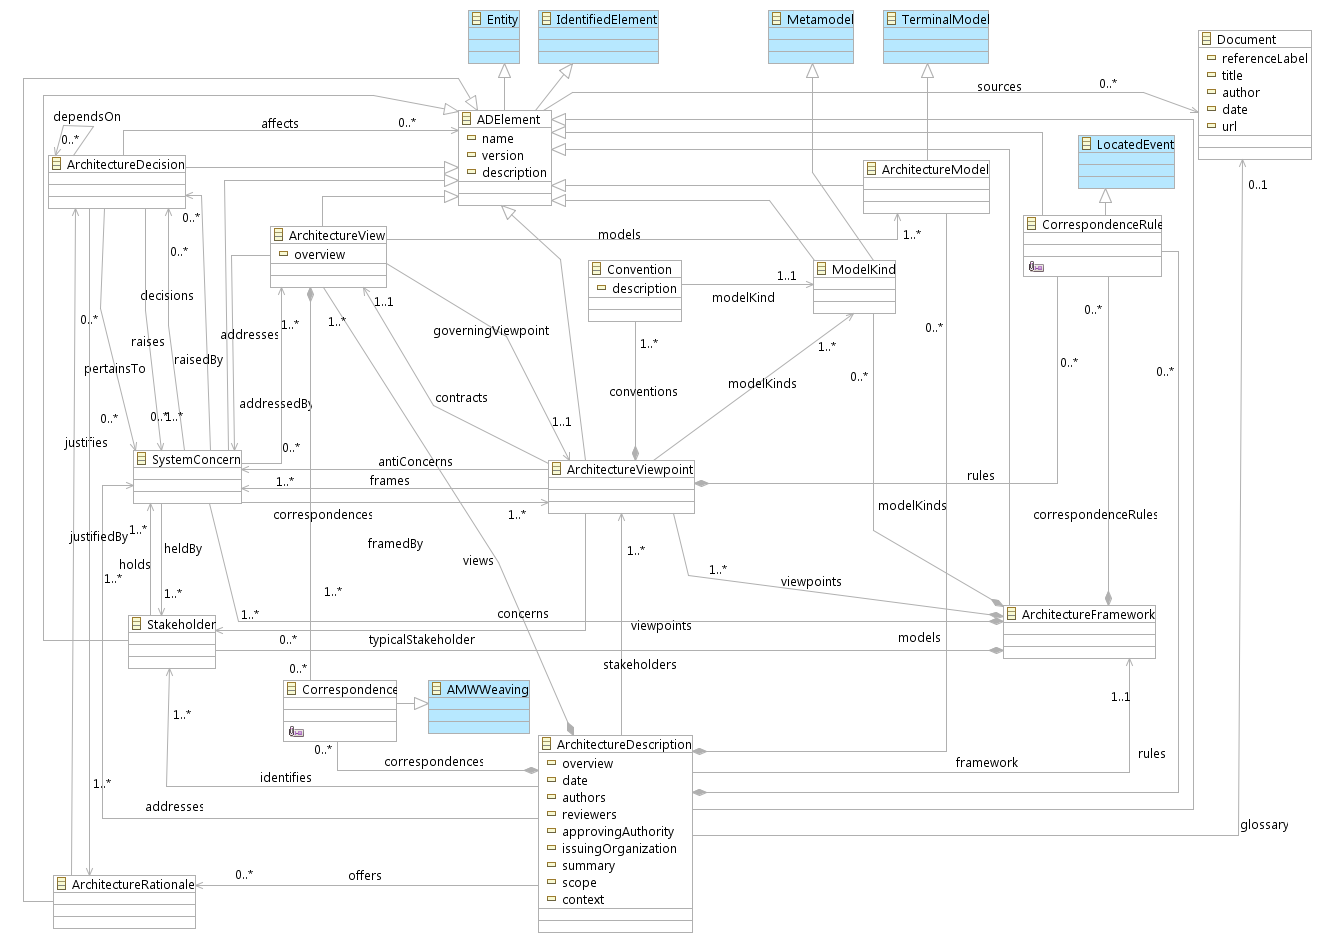
\includegraphics[width=\textwidth]{GMM4SA.png}
\caption{The GMM4SA meta-model}

\label{figure:GMM4SA}
\end{figure}

Architecture frameworks as defined by the \textit{ISO/IEC 42010 Software and System Engineering – Architecture Description} \cite{ISO/IEC42010} standard are collections of coordinated viewpoints, conventions, principles and practices to create architecture descriptions for specific stakeholders. Where \textit{architecture viewpoints} are collections of conventions, notations and modeling practices used to create concrete views which address domain specific system concerns for a distinct set of stakeholders. Their purpose is to capture and formalize a certain perspective.

According to the creators of MEGAF such architecture descriptions or frameworks alone have proven to be difficult to re-use and validate (consistency check). So in order to fix those issues, MEGAF shall provide features to: 
\begin{itemize}

\item 
\textit{store} architecture description elements (i.e. viewpoints, views, stakeholders, models, etc.), therefore making such elements reusable

\item
\textit{define correspondence relations and correspondence rules} between architecture description elements

\item
\textit{enable correctness and completeness checks} for architecture descriptions elements

\end{itemize}

To utilize mega-modeling techniques the assumption is made, that any architecture description element may conform to its meta-model. So a view may conform to a viewpoint, an architecture model may conform to a model kind, etc. This is straight forward and complies with the MDE world. The core of MEGAF is specified in \textit{Global Model Management for Software Architecture} (GMM4SA\footnote{\url{http://megaf.di.univaq.it/images/GMM4SA.png}}) meta-model shown in figure \ref{figure:GMM4SA} as UML class diagram. 

The diagram can be used to study the possible traceability of MEGAF. Because it is written in UML syntax, UML semantics apply and we already can identify several traceability links known from the MDE-Mega-Model. For example:
{\small \texttt{ArchitectureFramework} $\delta$ \texttt{ArchitectureViewpoint}} or {\small \texttt{ArchitectureViewpoint} $\varepsilon$ \texttt{ADElement}}.
These relations exist inherent in class diagrams as association/aggregation/composition ($\delta$) and generalization\footnote{UML generalization and realization do not map precisely to $\varepsilon$ and $\chi$ . The meaning may vary with the employed perspective. The set theoretic perspective ($\varepsilon$) might be used for data modeling. The model-meta-model perspective ($\chi$) might be used to describe inheritance or interface realization.} ($\varepsilon, \chi$). But this is trivial traceability information. The more beneficial traceability information here lies within the modeled context and intention. Because architecture description elements (children of \texttt{ADElement}) are formalizations of development process artifacts, all specified associations define a concrete traceability relation.

Lets consider the \texttt{ArchitectureViewpoint} class and its relations. In figure \ref{figure:GMM4SA} we see on the right hand side that \texttt{ArchitectureViewpoint} $\delta$ \texttt{Convention} and \texttt{ArchitectureViewpoint} $\delta$ \texttt{ModelKind}. Those are hard facts and can be interpreted as \textit{functional traces}. However on the left hand side wee see that an \texttt{ArchitectureViewpoint} \textit{frames} a \texttt{SystemConcern}. In the object oriented programming way of understanding such diagrams we would say \textit{frames} $\equiv \delta$. But if we also take the modeled context and intention of MEGAF into account, we discover how a \texttt{SystemConcern} traces to its holding \texttt{Stakeholder}, its pertaining \texttt{ArchitectureDecision} and the justifying \texttt{ArchitectureRationale}. Now we have information about \textit{reason, context and decision} and a successful formalization of \textit{non-functional traces}.

Wee see, the MEGAF meta-model supports traceability. Furthermore MEGAF and architecture frameworks in general target an very early phase of the development process. Using the higher order classification by Paige et. al \cite{}, MEGAF enables \textit{pre-model} traceability. However we need to note that pre-model traceability is concerned with non-model- to early-model-artifact traceability. On the other hand MEGAF seems to heavily discourage the use of non-model-artifacts at all. 


\subsection{Dynamic hierarchical mega-models \& Models at Runtime}
\subsection{Linguistic Architecture Analysis with MegaL}
MegaL\cite{MEGAL1}\cite{MEGAL2} is an approach on system understanding mainly concerned with the \textit{linguistic architecture} of the system under study. It intents to uncover the systems technological footprint by revealing the used technological spaces and their interrelations. This is called a \textit{linguistic} architecture because technological spaces of great interest are programming languages and their associated products.

In order to conduct a sufficient analysis MegaL needs to process the studied system against the 